\documentclass{article}
\listfiles
\usepackage{tikz}\usetikzlibrary{positioning,fit,arrows.meta}

\begin{document}
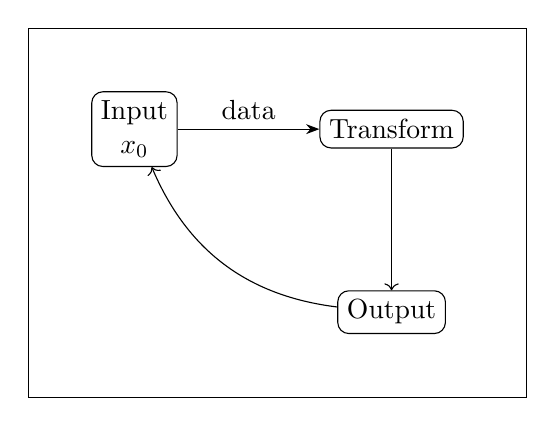
\begin{tikzpicture}[node distance=18mm,box/.style={draw,rounded corners,align=center}]
\node[box] (a) {Input\\$x_0$};\node[box,right=of a] (b) {Transform};\node[box,below=of b] (c) {Output};
\draw[-{Stealth}] (a)--node[above]{data}(b);\draw[->] (b)--(c);\draw[->,bend left] (c) to (a);
\node[draw,fit=(a)(b)(c),inner sep=8mm] {};
\end{tikzpicture}

\begin{tikzpicture}\foreach \x in {0,...,4}{\node[circle,draw] at (\x,0) {$\x$};}\end{tikzpicture}
\end{document}
